\section{线性表示中的拟合}
\label{sec:opt-fit-linear}

上一节的目标~\eqref{eq:opt-fit-general-objective}以函数为未知量。最直接的计算办法，是事先固定有限个基函数，只让它们的系数变化。这样函数拟合就变成有限维参数的优化：二次目标归结为一个最小二乘问题，可以直接调用线性代数中的分解与迭代求解器；稳健残差代价则可以借助逐轮构造的二次上界，变成一串加权最小二乘。

\subsection{线性基函数与二次正则化}
\label{sec:opt-fit-linear-basis}

\paragraph{设计矩阵与正则矩阵}
取$d$个基函数$\varphi_1,\dots,\varphi_d$，候选写成$f_{\bm w}=\sum_{j=1}^dw_j\varphi_j$。线性观测作用在它上面，得到
\[
  L_if_{\bm w}=\sum_{j=1}^dw_jL_i\varphi_j=(\bm X\bm w)_i,\qquad \bm X_{i,j}=L_i\varphi_j,
\]
称$\bm X\in\mathbb R^{n\times d}$为\term{设计矩阵}（design matrix），残差为$\bm X\bm w-\bm y$。点值观测时$\bm X_{i,j}=\varphi_j(x_i)$，就是熟悉的“特征矩阵”；积分观测时$\bm X_{i,j}$是基函数的积分。正则化同样由基函数算出：若$R(f)=\langle f,f\rangle$由某个内积给出，则$R(f_{\bm w})=\bm w^\top\bm R\bm w$，其中$\bm R_{j,k}=\langle\varphi_j,\varphi_k\rangle$；导数半范数$\int(f')^2$对应$\bm R_{j,k}=\int\varphi_j'\varphi_k'$，章首图中的曲率惩罚对应$\bm R_{j,k}=\int\varphi_j''\varphi_k''$。只有当基函数在相应内积下标准正交时，$\bm R$才是单位矩阵，函数范数才等于系数的欧氏范数。

\paragraph{同一数据上三种惩罚的选择}
取基$\{1,x\}$，只读到一个值$f(\tfrac12)=1$，于是$\bm X=(1,\tfrac12)$，一次函数$w_1+w_2x$中凡满足$w_1+w_2/2=1$的都插值数据。在这条直线上按三种惩罚选最小者。导数半范数$\bm R=\operatorname{diag}(0,1)$选出$w_2=0$，即常数$f=1$。$L^2$范数$\bm R=\bigl[\begin{smallmatrix}1&1/2\\1/2&1/3\end{smallmatrix}\bigr]$，由Lagrange条件，最小点与$\bm R^{-1}\bm X^\top=(1,0)^\top$成比例，也是常数$f=1$。系数欧氏范数$\bm R=\bm I$则选出与$\bm X^\top=(1,\tfrac12)^\top$成比例的点，即$\bm w=(\tfrac45,\tfrac25)$，$f(x)=\tfrac45+\tfrac25x$。三种惩罚在同一读数下给出两种不同的函数，而系数范数的选择会随基的改变而改变。

\paragraph{增广最小二乘}
设读数权重$\omega_i>0$给定，记$\bm\Omega=\operatorname{diag}(\omega_1,\dots,\omega_n)$，正则矩阵$\bm R$对称半正定，$\lambda>0$。拟合目标是
\begin{equation}
  \min_{\bm w\in\mathbb R^d}\ \frac12\bigl\|\bm\Omega^{1/2}(\bm X\bm w-\bm y)\bigr\|_2^2+\frac\lambda2\bm w^\top\bm R\bm w .
  \label{eq:opt-fit-quadratic}
\end{equation}
把$\bm R$分解为$\bm R=\bm B^\top\bm B$（例如Cholesky分解或对称平方根），惩罚就是$\tfrac\lambda2\|\bm B\bm w\|_2^2$，于是式~\eqref{eq:opt-fit-quadratic}等价于\term{增广最小二乘}（augmented least squares）
\begin{equation}
  \min_{\bm w}\ \frac12\left\|\begin{bmatrix}\bm\Omega^{1/2}\bm X\\ \sqrt\lambda\,\bm B\end{bmatrix}\bm w-\begin{bmatrix}\bm\Omega^{1/2}\bm y\\ \bm 0\end{bmatrix}\right\|_2^2,
  \label{eq:opt-fit-augmented}
\end{equation}
其正规方程为$(\bm X^\top\bm\Omega\bm X+\lambda\bm R)\bm w=\bm X^\top\bm\Omega\bm y$。$\bm R=\bm I$、$\bm\Omega=\bm I$时，这就是\term{岭回归}（ridge regression），也称\term{Tikhonov正则化}（Tikhonov regularization）。

\paragraph{唯一性由共同零方向决定}
最小二乘问题~\eqref{eq:opt-fit-augmented}的解唯一，当且仅当增广矩阵列满秩，即它的零空间只含零向量。增广矩阵作用在$\bm w$上为零，等价于$\bm\Omega^{1/2}\bm X\bm w=\bm 0$且$\bm B\bm w=\bm 0$；由$\omega_i>0$，前者即$\bm X\bm w=\bm 0$；由$\bm w^\top\bm R\bm w=\|\bm B\bm w\|_2^2$与$\bm R\succeq\bm 0$，后者即$\bm R\bm w=\bm 0$。所以
\[
  \text{式~\eqref{eq:opt-fit-quadratic}的解唯一}\iff\ker\bm X\cap\ker\bm R=\{\bm 0\}.
\]
读数看不见的方向，只要惩罚能看见，就被惩罚确定；两者都看不见的方向，目标值沿它不变，解就不唯一。上面的例子中，$\ker\bm X=\operatorname{span}\{(1,-2)^\top\}$，导数半范数的$\ker\bm R=\operatorname{span}\{(1,0)^\top\}$，两者只交于零，所以即使惩罚本身是半范数，解也唯一。

\paragraph{岭回归的谱滤波}
$\bm R=\bm I$时，借助奇异值分解可以看清正则化对每个方向做了什么。设$\bm X=\sum_{k=1}^r\sigma_k\bm u_k\bm v_k^\top$，$\sigma_k>0$。正规方程$(\bm X^\top\bm X+\lambda\bm I)\bm w=\bm X^\top\bm y$在基$\{\bm v_k\}$下逐坐标解开，得到
\begin{equation}
  \bm w_\lambda=\sum_{k=1}^r\frac{\sigma_k^2}{\sigma_k^2+\lambda}\cdot\frac{\bm u_k^\top\bm y}{\sigma_k}\,\bm v_k ,
  \label{eq:opt-fit-ridge-svd}
\end{equation}
零奇异值方向（即$\ker\bm X$）的系数为零。$\bm u_k^\top\bm y/\sigma_k$是不加正则时沿$\bm v_k$的最小二乘系数，前面的因子$\sigma_k^2/(\sigma_k^2+\lambda)$称为\term{滤波因子}（filter factor）。图~\ref{fig:opt-fit-ridge-filter}显示，它在$\sigma_k\gg\sqrt\lambda$时接近$1$，几乎不改变该方向；在$\sigma_k\ll\sqrt\lambda$时近似为$\sigma_k^2/\lambda$，把该方向压到接近零；过渡发生在$\sigma_k=\sqrt\lambda$附近，那里恰好保留一半。小奇异值方向上的最小二乘系数$\bm u_k^\top\bm y/\sigma_k$会把读数的微小变化放大$1/\sigma_k$倍，岭回归削弱的正是这些方向。

\begin{figure}[!htbp]
  \centering
  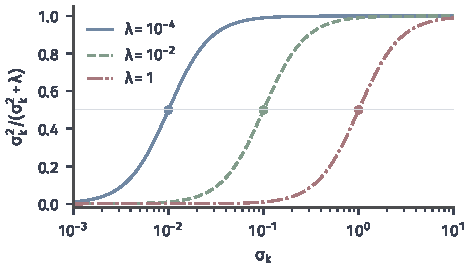
\includegraphics[width=80mm]{figures/03-optimization-evolution-and-signals/01-optimization/matplotlib/c8-ridge-filter/figure.pdf}
  \caption{岭回归在奇异值方向上的滤波因子$\sigma_k^2/(\sigma_k^2+\lambda)$，横轴为对数刻度，$\lambda=10^{-4},10^{-2},1$。圆点标出$\sigma_k=\sqrt\lambda$处因子恰为$\tfrac12$；大于$\sqrt\lambda$的奇异值方向基本保留，小于$\sqrt\lambda$的方向被压向零。}
  \label{fig:opt-fit-ridge-filter}
\end{figure}

\paragraph{求解器的选择}
式~\eqref{eq:opt-fit-augmented}是标准的线性最小二乘问题，QR分解、奇异值分解、LSQR等求解方法及伪逆与最小范数解的性质，可参考\BookChapterRef{chap:linear-equations-and-optimization}{卷一“线性方程与矩阵方程”章}；这里只说明怎样按问题结构选用。矩阵规模中等、增广矩阵列满秩时，对它做QR分解最稳妥，避免显式形成正规方程，后者会把条件数平方。要对许多个$\lambda$求解，或$\bm X$接近秩亏时，先做一次奇异值分解，再由式~\eqref{eq:opt-fit-ridge-svd}对每个$\lambda$只花$O(rd)$的代价组合系数。$\bm X$大而稀疏、只能做矩阵向量乘积时，用LSQR一类的Krylov方法直接作用于增广系统，它们原生支持“阻尼”项$\sqrt\lambda\bm I$，每轮只需一次$\bm X\bm v$与一次$\bm X^\top\bm u$。

\subsection{稳健拟合与迭代重加权最小二乘}
\label{sec:opt-fit-irls}

平方代价把远离其他读数的点看得很重。图~\ref{fig:opt-fit-irls}(a)中十四个点大致沿直线$y=1+2x$分布，其中两点被人为下移了两个多单位；普通最小二乘直线被它们拉得几乎放平，斜率只有$0.71$。换用对大残差增长较慢的代价可以减轻这种影响，但目标不再是二次的。本小节说明，对一类常用的稳健代价，可以逐轮构造一个二次上界，把问题化成一串加权最小二乘。

\paragraph{从残差平方的凹函数出发}
固定线性残差$r_i(\bm w)=\bm X_{i,:}\bm w-y_i$，把目标写成残差平方的函数
\begin{equation}
  F(\bm w)=\frac12\sum_{i=1}^n\rho\bigl(r_i(\bm w)^2\bigr),
  \label{eq:opt-fit-robust-objective}
\end{equation}
其中$\rho:[0,\infty)\to\mathbb R$可微、非减，并且对平方残差$s=r^2$是凹函数。平方代价对应$\rho(s)=s$；Huber损失对应$\rho(s)=s$（$s\le\delta^2$）与$\rho(s)=2\delta\sqrt s-\delta^2$（$s>\delta^2$）；Cauchy代价对应$\rho(s)=c^2\log(1+s/c^2)$，$c>0$为尺度。它们的导数$\rho'(r^2)$分别是$1$、$\min\{1,\delta/|r|\}$与$1/(1+r^2/c^2)$，正是图~\ref{fig:opt-fit-residual-losses}(b)中的权重曲线。绝对值代价对应$\rho(s)=2\sqrt s$，在$s=0$处不可微，权重$1/|r|$在零残差处无界，不满足这里的条件。

\paragraph{切线给出二次上界}
凹函数位于它任一点的切线之下：对$s,s_0\ge0$，$\rho(s)\le\rho(s_0)+\rho'(s_0)(s-s_0)$。在当前点$\bm w^{(t)}$处记$s_i^{(t)}=r_i(\bm w^{(t)})^2$，令\emph{权重}
\[
  \gamma_i^{(t)}=\rho'\bigl(s_i^{(t)}\bigr)\ge0,
\]
非负性来自$\rho$非减。把切线不等式用于每个$s=r_i(\bm w)^2$并求和，得到
\begin{equation}
  F(\bm w)\le Q(\bm w\mid\bm w^{(t)})
  =\frac12\sum_{i=1}^n\Bigl[\rho\bigl(s_i^{(t)}\bigr)+\gamma_i^{(t)}\bigl(r_i(\bm w)^2-s_i^{(t)}\bigr)\Bigr],
  \label{eq:opt-fit-irls-surrogate}
\end{equation}
且$\bm w=\bm w^{(t)}$时两边相等。$Q$关于$\bm w$是加权平方和加常数，所以极小化它就是解一个\term{加权最小二乘}（weighted least squares）问题。这正是第~\ref{chap:opt-nonsmooth}章主化--最小化（MM）方法的构造：代理在全域位于原目标之上、在当前点与之相切，于是对代理的任何改善都传给原目标，
\[
  F(\bm w^{(t+1)})\le Q(\bm w^{(t+1)}\mid\bm w^{(t)})\le Q(\bm w^{(t)}\mid\bm w^{(t)})=F(\bm w^{(t)}).
\]
权重必须由同一个$\rho$在当前残差处求导得到；若随意重设权重，代理就不再是$F$的上界，这条不等式链随之失效。

\begin{algorithm}[迭代重加权最小二乘]
\label{alg:opt-fit-irls}
\begin{algorithmic}[1]
\Require 设计矩阵$\bm X$、读数$\bm y$、满足上述条件的$\rho$、初值$\bm w^{(0)}$、容许误差$\epsilon>0$、最大轮数$T$
\Ensure 参数$\bm w$及其目标值$F(\bm w)$
\For{$t=0,1,\dots,T-1$}
  \State 计算残差$r_i=\bm X_{i,:}\bm w^{(t)}-y_i$与权重$\gamma_i=\rho'(r_i^2)$，记$\bm\Gamma=\operatorname{diag}(\gamma_i)$
  \State 以QR或SVD求解$\min_{\bm w}\|\bm\Gamma^{1/2}(\bm X\bm w-\bm y)\|_2^2$，得候选$\tilde{\bm w}$
  \State 若$Q(\tilde{\bm w}\mid\bm w^{(t)})>Q(\bm w^{(t)}\mid\bm w^{(t)})$，报告子问题求解失败并停止
  \State $\bm w^{(t+1)}\gets\tilde{\bm w}$
  \If{$F(\bm w^{(t)})-F(\bm w^{(t+1)})\le\epsilon\,(1+F(\bm w^{(t)}))$}
    \State \Return $\bm w^{(t+1)}$
  \EndIf
\EndFor
\State \Return $\bm w^{(T)}$
\end{algorithmic}
\end{algorithm}

算法~\ref{alg:opt-fit-irls}称为\term{迭代重加权最小二乘}（iteratively reweighted least squares，IRLS）。每轮的主要代价是一次$n\times d$的加权最小二乘，用QR分解约为$O(nd^2)$；把$\sqrt{\gamma_i}$乘到$\bm X$与$\bm y$的第$i$行上，就能直接调用普通最小二乘求解器。第4步的检查不是多余的：当子问题只被近似求解时，只有代理确实不增，上面的下降链才成立。

\begin{example}[用常数拟合$0,0,10$]
\label{ex:opt-fit-irls-cauchy}
取$\bm X=(1,1,1)^\top$，$\bm y=(0,0,10)^\top$，Cauchy代价$c=1$，即$F(w)=\tfrac12\sum_i\log(1+(w-y_i)^2)$，初值$w^{(0)}=0$。残差为$0,0,-10$，权重$\gamma_i=1/(1+r_i^2)$依次为$1,1,1/101$。加权最小二乘的解是加权平均
\[
  w^{(1)}=\frac{1\cdot0+1\cdot0+\tfrac1{101}\cdot10}{1+1+\tfrac1{101}}=\frac{10}{203}\approx0.0493 .
\]
目标值从$F(0)\approx2.3076$降到$F(w^{(1)})\approx2.3051$。重算权重后继续迭代，序列很快稳定在$w\approx0.0499$。远处的读数$10$只得到约$1/100$的权重，几乎不影响结果，这与均值$10/3$形成对照。
\end{example}

图~\ref{fig:opt-fit-irls}(b)画出了这个例子的原目标与首轮代理：黄色虚线是$w^{(0)}=0$处构造的二次函数，它处处位于蓝色曲线之上，在$w=0$处与之相切，其最小点$10/203$就是红点所示的新迭代。同一图还暴露出$F$的非凸性：在$w\approx9.79$处另有一个局部最小点，目标值约$4.59$，远高于$2.31$。若从$w^{(0)}=10$出发，权重变为$1/101,1/101,1$，IRLS会停在这个局部最小点。代理下降只保证目标不增，不保证找到非凸目标的全局最小点；初值通常取普通最小二乘解或其他稳健的粗估计。

\begin{figure}[!htbp]
  \centering
  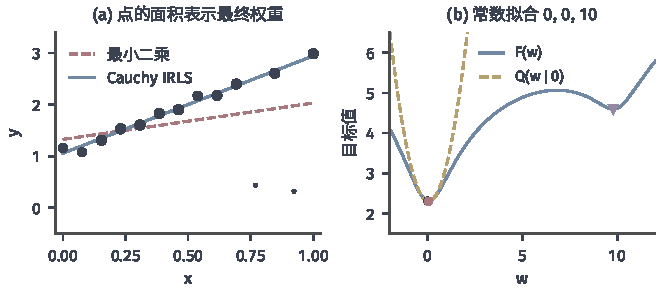
\includegraphics[width=112mm]{figures/03-optimization-evolution-and-signals/01-optimization/matplotlib/c8-irls-outliers/figure.pdf}
  \caption{稳健拟合与迭代重加权。(a)~教学示例数据：$14$个点$y=1+2x$加固定种子的小噪声，其中两点下移$2.2$与$2.6$。红色虚线为普通最小二乘直线（截距$1.33$、斜率$0.71$）；蓝线为Cauchy代价（$c=0.2$）的IRLS结果（截距$1.06$、斜率$1.89$）；点的面积正比于最终权重，两个离群点的权重约为$0.009$与$0.006$，其余点不低于$0.71$。(b)~用常数$w$拟合$0,0,10$的Cauchy目标$F(w)$（$c=1$，蓝线）与$w^{(0)}=0$处的代理$Q(w\mid0)$（黄色虚线）；黑点为初值，红点为首轮更新$10/203$，紫色三角为$w\approx9.79$处的局部最小点。}
  \label{fig:opt-fit-irls}
\end{figure}

\paragraph{权重退化、子问题误差与永久正则}
三种情形需要在实现中单独处理。第一，有些代价（例如在阈值外权重恰为零的Tukey双权代价）会给大残差零权重；若权重为零的行太多，使$\bm\Gamma^{1/2}\bm X$不再列满秩，加权最小二乘不唯一，此时应取最小范数解或检查初值与尺度，而不是任意选一个解。对绝对值代价，常用的补救是把权重改为$1/\max\{|r_i|,\epsilon\}$，但这相当于换成了一个光滑化的目标，结论要对新目标陈述。第二，子问题用迭代法近似求解时，按算法第4步检验代理值。第三，若原问题本身含正则项，例如$F(\bm w)+\tfrac\lambda2\|\bm w\|_2^2$，这一项不需要线性化，应原样加进每一轮的代理，于是每轮求解的是带同一$\lambda$的增广最小二乘~\eqref{eq:opt-fit-augmented}；它是目标的一部分，与下一节为控制步长而临时加入的阻尼不同。
